% mnras_template.tex 
%
% LaTeX template for creating an MNRAS paper
%
% v3.0 released 14 May 2015
% (version numbers match those of mnras.cls)
%
% Copyright (C) Royal Astronomical Society 2015
% Authors:
% Keith T. Smith (Royal Astronomical Society)

% Change log
%
% v3.0 May 2015
%    Renamed to match the new package name
%    Version number matches mnras.cls
%    A few minor tweaks to wording
% v1.0 September 2013
%    Beta testing only - never publicly released
%    First version: a simple (ish) template for creating an MNRAS paper

%%%%%%%%%%%%%%%%%%%%%%%%%%%%%%%%%%%%%%%%%%%%%%%%%%
% Basic setup. Most papers should leave these options alone.
\documentclass[fleqn,usenatbib]{mnras}


% MNRAS is set in Times font. If you don't have this installed (most LaTeX
% installations will be fine) or prefer the old Computer Modern fonts, comment
% out the following line
\usepackage{newtxtext,newtxmath}
\usepackage{anyfontsize}
% Depending on your LaTeX fonts installation, you might get better results with one of these:
%\usepackage{mathptmx}
%\usepackage{txfonts}

% Use vector fonts, so it zooms properly in on-screen viewing software
% Don't change these lines unless you know what you are doing
\usepackage[T1]{fontenc}

% Allow "Thomas van Noord" and "Simon de Laguarde" and alike to be sorted by "N" and "L" etc. in the bibliography.
% Write the name in the bibliography as "\VAN{Noord}{Van}{van} Noord, Thomas"


%%%%% AUTHORS - PLACE YOUR OWN PACKAGES HERE %%%%%

% Only include extra packages if you really need them. Common packages are:
\usepackage{graphicx}	% Including figure files
\usepackage{amsmath}	% Advanced maths commands
% \usepackage{amssymb}	% Extra maths symbols

\usepackage{isotope}

\usepackage{hyperref}

\graphicspath{{figures/}} 




%%%%%%%%%%%%%%%%%%%%%%%%%%%%%%%%%%%%%%%%%%%%%%%%%%

%%%%% AUTHORS - PLACE YOUR OWN COMMANDS HERE %%%%%

% Please keep new commands to a minimum, and use \newcommand not \def to avoid
% overwriting existing commands. Example:
%\newcommand{\pcm}{\,cm$^{-2}$}	% per cm-squared


% citations
\defcitealias{james+21}{J21}
\newcommand{\JJ}{\citetalias{james+21}}
\newcommand{\VICE}{\textsc{vice}}
\newcommand{\citetjack}{Roberts et al.~(2023, in prep.)}
\newcommand{\citepjack}{(Roberts et al.~2023, in prep.)}
\newcommand{\citealtjack}{Robert et al.~2023, in prep.}
\newcommand{\cxi}{\texttt{\hyperlink{C11}{C11}}}
\newcommand{\kx}{\texttt{\hyperlink{K10}{K10}}}
\newcommand{\kxvi}{\texttt{\hyperlink{K16}{K16}}}
\newcommand{\vxiii}{\texttt{\hyperlink{V13}{V13}}}



% Acronyms
\newcommand{\agb}{AGB}
\newcommand{\apogee}{APOGEE}
\newcommand{\cc}{CCSNe}
\newcommand{\gce}{GCE}
\newcommand{\ia}{SNe Ia}
\newcommand{\imf}{IMF}
\newcommand{\sfh}{SFH} % check where first defined
\newcommand{\ssp}{SSP}

% internal abbreviations
\newcommand{\lims}{lower-intermediate mass stars}
\newcommand{\hms}{high-mass stars}
\newcommand{\caah}{[C/Mg]-[Mg/H]}
\newcommand{\caafe}{[C/Mg]-[Mg/Fe]}

% other
\makeatletter
\newcommand{\C}[1][\@nil]{
    \def\tmp{#1}%
    \ifx\tmp\@nnil%
        \ensuremath{\rm C}%
    \else%
        \ifmmode ^{#1}{\rm C}%
        \else $^{#1}$C%
        \fi%
\fi }
\makeatother

\newcommand{\Yct}{\ensuremath{y_{\rm C}}}
\newcommand{\Ycc}{\ensuremath{y_{\rm C}^{\rm cc}}}
\newcommand{\Yoc}{\ensuremath{y_{\rm Mg}^{\rm cc}}}
\newcommand{\Ycagb}{\ensuremath{y_{\rm C}^{\rm agb}}}
\newcommand{\y}{\ensuremath{\rotatebox[origin=B,y=0.5ex]{180}{y}}}

\newcommand{\Mo}{%
    \ifmmode {\rm M}_{\sun}%
    \else M$_{\sun}$
    \fi}
\newcommand{\Zo}{%
    \ifmmode Z_{\sun}%
    \else $Z_{\sun}$%
    \fi}

\newcommand{\about}[1]{${\sim} #1$}

%%%%%%%%%%%%%%%%%%%%%%%%%%%%%%%%%%%%%%%%%%%%%%%%%%

%%%%%%%%%%%%%%%%%%% TITLE PAGE %%%%%%%%%%%%%%%%%%%

% Title of the paper, and the short title which is used in the headers.
% Keep the title short and informative.
\title[The Origin and Galactic Evolution of Carbon]{The Galactic Chemical Evolution of Carbon: Implications for Stellar Nucleosynthesis }

% The list of authors, and the short list which is used in the headers.
% If you need two or more lines of authors, add an extra line using \newauthor
\author[D. A. Boyea et. al.]{
Daniel A. Boyea,$^{1}$\thanks{E-mail: boyea.2@osu.edu}
James W. Johnson,$^{1}$
Third Author$^{2,3}$
and Others$^{1,3}$
\\
% List of institutions
$^{1}$Department of Astronomy, the Ohio State University, 191 W. Woodruff, Columbus, OH 43210, USA
}

% These dates will be filled out by the publisher
\date{Accepted XXX. Received YYY; in original form ZZZ}

% Enter the current year, for the copyright statements etc.
\pubyear{2023}

% Don't change these lines
\begin{document}
\label{firstpage}
\pagerange{\pageref{firstpage}--\pageref{lastpage}}
\maketitle



% Abstract of the paper
\begin{abstract}
% context
C is an important element across astronomy. However, its origin remains poorly understood. 
% 
As stellar yields are highly uncertain, we aim to constrain the stellar yields of C through multi-zone Galactic chemical evolution models. 
% results
We use \apogee\ subgiants to constrain the model. 
% 
We find that \caafe\ is an emirical estimate of the delayed C sources, enabling us to estimate that \agb\ stars and \cc\ produce about 20\% and 80\% of C, respectively.  
The \caah\ trend instead represents the equilibrium abundances of C and Mg. 
We use the \caah\ trend to estimate the CCSNe C/Mg yield, determining that  $\Ycc/\Yoc = EQUATION$ when including \agb\ C. 
% misc
Our models are relatively independent of uniform scaling of yields and outflows, and alternate star formation histories. 
However, the stars which contribute to \agb\ C production and the \ia\ delay time distribution of Fe contribute uncertainties to our conclusions. 
% gas phase
While reliable gas-phase and low-metallicity measurments of C are challenging, we find that our model and a singlezone model with our recommended yields replicate the broad trends of \caah across different environments and metallicities. 

\end{abstract}





%%%%%%%%%%%%%%%%%%%%%%%%%%%%%%%%%%%%%%%%%%%%%%%%%%

%%%%%%%%%%%%%%%%% BODY OF PAPER %%%%%%%%%%%%%%%%%%

\section{Introduction}

Carbon is a distinctive and well-studied element in astronomy. 
Formed in the cores of stars during He fusion, C is the lightest directly synthesized element after He, one of the only light elements formed in low-mass stars, and one the most abundant metals\footnotemark{}. % \citep[e.g.][]{jennifer19, KL14}
C structurally changes the environments it pollutes, modifying stellar evolution, facilitating the formation of stars and planets, and forming the basis of earthly life.
% C/N as age indicator?
As such, understanding the origin of C has wide ranging implications. 
While we know both lower-intermediate-mass and high-mass stars produce C, the relative importance of each process is still unknown.

\footnotetext{Astronomers are not chemists. By metallicity, we mean the (mass) fraction of any element which is not H or He, denoted by $Z$. For the sun, $Z_\odot=0.014$. }


Galactic chemical evolution is a powerful tool in understanding the origin of elements. 
Each enrichment process has distinct chemical signatures and timescales, enabling us to reconstruct chemical histories.
Many previous works have used GCE in attemt to understand C abundances, whether through using theoretical stellar models \citep{DTS78, prantzos+18, chiappini+03} 
or understanding  observation \citep{tinsley79, HEK00, BF06, rybizki+17, berg+19, KKL20}.
(See also review in \citealt{romano22}.)
%
Every study agrees that C is produced by a combination of high-mass and \lims{}, different studies disagree on which process is dominant. 
For example CITES conclude \hms{} dominate wherease CITES conclude \lims{} contribute the majority of C.
C is also generally understood to have strong metalliicity dependent CCSNe enrichment. 


One of the primary uncertainties of GCE models are nucleosynthetic yields. Yield predictions -- the amounts of each chemical element stars produce --
are shaped by poorly understood processes, including mass loss, nuclear reaction rates, rotational mixing, convection, and explodability \citep{romano+10,KL14,ventura+13, LC18, emily+21}.
To better understand where C comes from and how it evolves, our aim is to use a combination of \apogee\ observations and multi-zone models to develop estimates of the required C yields to reproduce galactic trends.
\cite{james+23} examined similar \gce{} models of N (which is closely related to C), finding that trends in N and O\footnotemark{} are explained by the metallicity dependence of N/O yields. \citet{james+23} determine that \agb\ N abundances roughly dependence on metallicity (i.e. $y_{\rm N}/y_{\rm O} \propto Z$). 
Here, we extend their models to C, deriving similar constraints on C/Mg yields. We assess which yield prescriptions reproduce Galactic abundance trends while investigating the impact of \gce{} model assumptions, such as the star formation history (\sfh{}) and outflow mass loading.

 
\footnotetext{e.g. \citet{HEK00,PVT10,berg+12, berg+20, skillman+20, izotov+12, james2+15, dopita+16}.} 
We know, from observations of MW stars and extragalactic gas measurments, that C/O traces a banana shape in O/H (see \ref{fig:gas_phase}). 
% \cite[e.g.][]{fabbian+09, nissen+14, lambert81, laird85, lambert86}. 
At very low metallicities, C/O decreases with increasing metallicity, from observations of halo stars and damped Lyman-alpha systems\footnotemark{} \citep{nissen+14, cooke+17, fabbian+09}. 
\footnotetext{DLAs; high redshift clouds of gas observed as absorption lines in yet higher redshift quasars}
%
However, the trend reverses around $[{\rm O/H}]\approx-1$\footnotemark{}. 
C/O instead increases with increasing metallicity in observations of HII regions and Milky Way stars (\citealt{berg+19}; see discussion in section \ref{sec:gas}).


\footnotetext{In this paper, we use the standard notation for chemical abundances. $[A/B] = \log_{10}\left(A/B\right) - \log_{10}\left(A_{\sun}/B_{\sun}\right)$, i.e. $[A/B]$ is the logarithm of the ratio between A and B, scaled such that $[A/B]=0$ for the sun. Solar abundances are as measured in \citet{asplund+09}.}


However, observations of C are not without challenges. 
As stars ascend the red giant branch (RGB) at the end of H core burning, C abundances are changed by \textit{first dredge up}\footnotemark{}. This has the benefit of allowing C/N to be used as an age indicator in RGB stars \citep{MG15, martig16, hasselquist19, vincenzo+21}, but evolved stars are no longer as useful for determining birth abundances. Works such as \citet{vincenzo+21} attempt to correct for these changes but this requires MESA stellar modeling. 
In optical spectroscopy, C lines are relatively faint, and surveys such as GALAH struggle against low detection rates, potentially biasing sample measurments. While \apogee\ includes more reliable C$_2$ lines, there is an additional risk of systematics because .....
In the gas phase, HII regions are our best window into C abundances in our galaxy and extragalactic regions including dwarf. 
Unfortunantly, C lacks strong optical emission lines. Approaches use either recombination lines or ... in the ultraviolet, but these methods disagree, making gas-phase abundances a limited metric for GCE models of C.


    As our primary observational constraint, we use a sample of subgiant stars from the \apogee{} \citep{apogee17}. selected by the criteria in Roberts et al. (2023, in prep; see Appendix \ref{sec:jack}).
According to stellar evolution theory and observations \citep{gilroy89, korn+07, lind+08, souto+18, souto19}, these stars have not yet experienced first dredge up (FDU) but have well-mixed envelopes. So, subgiant surface abundances should represent their birth composition. 
Fig.~\ref{fig:subgiants} shows the subgiant sample plotted in \caah\ and \caafe{}. [C/Mg] increases with metallicity, and [C/Mg] decreases with [Mg/Fe] at fixed [Mg/H]. 
Using these trends, we will develop a model of the enrichment sources and evolution of C.

\citet{james+23} compare their model against the \cite{vincenzo+21} sample of \apogee{} \citep{apogee17} RGB stars. \citet{vincenzo+21} use \textsc{mesa} stellar evolution models \citep{mesa} to correct for the effects of first dredge up. 
We instead use the \citetjack~sample of \apogee{} subgiants. Subgiant stars have not undergone first dredge up but have well-mixed atmospheres, so their atmospheric C and N abundances are still reflective of their birth abundances and do not need mixing corrections. We only compare the models to the low-$\alpha$ sequence unless otherwise specified.  The selection criteria and differences between the samples are described in more detail in Appendix \ref{sec:jack}.


\footnotetext{First dredge up (FDU) is when material from CNO processed core is mixed with the (convective) stellar envelop during the ascent onto the RGB. As a result, C is decreased and N is increased depending on the strength of this process and the envelop mass.}


\begin{figure*}
    \centering
    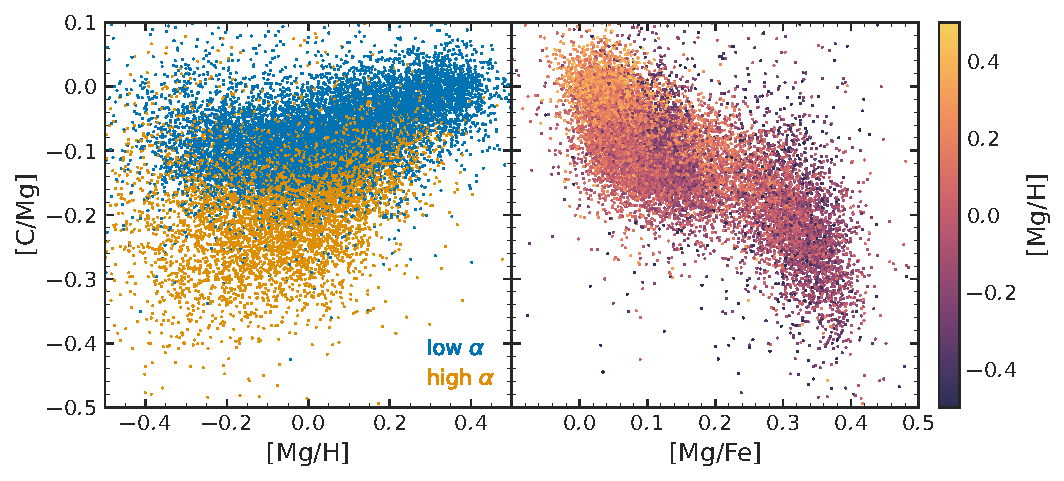
\includegraphics{subgiants.pdf}
    \caption{The [C/Mg] ratio against [Mg/H] (top) and [Mg/Fe] (bottom) for the \citetjack~sample of \apogee{} subgiants. On the top, we plot high and low-$\alpha$ stars in blue and orange, using the separation defined in Equation \ref{eq:high_alpha} (the high and low-$\alpha$ stars are named for their high or low $\alpha$-element to Fe ratios, or in this case, Mg/Fe). On the bottom, we colour-code stars according to their [Mg/H] abundance.} \label{fig:subgiants}
\end{figure*}








\section{Nucleosynthesis}

Yields -- the amounts of each chemical element stars synthesise -- are central to studies of galactic chemical evolution (GCE). 
In this section, we discuss the yield choices of our model and literature models for C yields. 
We focus on three nucleosynthetic pathways: asymptotic giant branch (\agb{}) stars, core collapse supernovae (\cc{}), and type Ia supernovae (\ia{}).
C is produced in both \agb{} and \cc{} stars.
We also use Mg and Fe as tracers of \cc{} and \ia{} enrichment respectively. 
O and Mg are produced almost entirely from \cc\ with metallicity-independent yields. In contrast Fe is produced in similar amounts by \cc\ and \ia.

After a single stellar population (SSP)\footnotemark{} forms, \cc{} are the first chemical enrichers. \cc{} explode within $\lesssim 40$\,Myr, providing light elements (e.g. C, O, and Mg) and heavier elements (Fe and beyond). Next, low-mass stars begin to reach the end of their lives, entering the \agb{} phase. By shedding their outer layers, \agb{} stars are important sources of C, N, and neutron capture elements.  Finally, white dwarfs explode in \ia{}, releasing Fe and other iron-peak elements.

\footnotetext{SSP: Single stellar population. Technical name for a group of stars born in the same conditions at the same time, i.e. an open cluster.}


To quantify yields, we define the stellar yield to be the fraction of a stars initial mass which is newly synthesized and released as a given element. 
For an element $X$ and star with mass $M$, the net-fractional stellar yield $\y$ is 
\begin{equation}
\y_{X} =  \Delta Z_X \frac{M_{\rm ejected}}{M_{\rm birth}}
\end{equation}
where $M_{\rm ejected}$ and $M_{\rm birth}$  are the total ejected mass and the birth mass of the star, and $\Delta Z_X$ is the change in $Z_X$ from the birth material to the ejected material of the star.%
\footnote{$Z_{X}$ represents the mass fraction of element $X$.}
%
For example, a 1\,\Mo\ star with $\y_{\C} = 10^{-3}$ will add $10^{-3}\,\Mo$ of new C to the interstellar medium. 
Also, note that yields may be negative if the material returned to the interstellar medium has a lower abundance $Z_X$ than the material the star was formed from.
Although per-star yields are necessary to compute \agb{} star enrichment rates in \gce{}  models, \imf-averaged yields are useful in interpreting their predictions. 
Given the fractional yield $\y(M, Z)$ as a function of initial stellar mass $M$ and metallicity $Z$, the \imf-averaged yield is given by 
\begin{equation} \label{eq:imf-yield}
    y_{\rm X}(Z,t) = 
    \frac{
    \int_{M_{\rm min}(t)}^{M_{\rm max}} 
    \y_{\rm X}(M, Z)
    \frac{dN}{dM}\ M\ dM
}
{
    \int \frac{dN}{dM}\ M\ dM
}
\end{equation}
where ${dN}/{dM}$ is the \imf, $M_{\rm max}=100\,\Mo$ is the maximum stellar mass, and $M_{\rm min}(t)$ is the mass of stars with lifetime $t$.\footnotemark{}
We use $t=10\,$Gyr for total yields when $t$ is not used.
To calculate the \imf-averaged net yields, we use the Versatile Integrator for Chemical Evolution code (\VICE).\footnotemark{} 

We adapt the yield choices of elements besides C from \citet{james+21, james+23}.
Table \ref{tab:fiducial_mod} contains our fiducial yields. 
Following \citet{james+21, james+23}, we also take the \ia{} delay time distribution to be a $t^{-1.1}$ power-law, as suggested by the observations of \citet{maoz+12}.

\addtocounter{footnote}{-2}
    \stepcounter{footnote}\footnotetext{In our model, the mass-lifetime relation is
$\log \tau_M = 1.02 - 3.57\log M + 0.90 \left(\log M\right)^2$,
where $\tau_M$ is in Gyr, from \citealt{larson74}}

\stepcounter{footnote}\footnotetext{\VICE~is available at \url{https://github.com/giganano/VICE}}

\begin{table}
	\centering
    \caption[]{Yields for the fiducial model (in units of \ssp~birth mass). See Section \ref{sec:agb} for the definition of \cxi.}
	\label{tab:fiducial_mod}

	\begin{tabular}{l l l l}
		\hline
        Element & $y^{\rm cc}$ & $\y^{\rm agb}$ & $y^{\rm ia}$ \\
		\hline
        C & Eq.~\ref{eq:zeta} & $2.9\times{\rm C11}$ &  0 \\
        O & 0.015 & 0 & 0 \\
        Mg & 0.00185 & 0 & 0 \\
        Fe & 0.0012 & 0 & 0.00214 \\
        N & 0.00072 & 0.0009$M\left(\frac{Z}{Z_\odot}\right)$ & 0\\
		\hline
	\end{tabular}
\end{table}

\subsection{Asymptotic Giant Branch Stars}\label{sec:agb}


An \agb\ star is a low-mass star ($\lesssim 8 M_{\sun}$) during its final phase of evolution.  
In an \agb\ star, two competing processes determine the outcome of C production: \textit{third dredge up} and \textit{hot bottom burning}.  
Third dredge up accompanies thermal pulses in \agb\ stars, where material from the CO core is mixed with the envelope, increasing surface C abundances \citep{KL14}. The C yields of the star are increased as this C-enhanced envelope is released to the interstellar medium. 
Hot bottom burning is the activation of the CNO cycle\footnotemark{}
at the bottom of the convective envelope when $T\gtrsim 50\,{\rm MK}$. Because the $^{14}$N proton capture is the slowest component of the CNO cycle, the CNO cycle converts nearly all \C[12] into $^{14}$N \citep{solar-fusion}.

\footnotetext{
    The CNO cycle is a series of proton-capture reactions with CNO elements resulting in energy generation and the creation of an $\alpha$ particle. $\C[12]({\rm p}, \gamma)
    ^{13}{\rm N}(\beta^+, \nu_{\rm e})
    ^{13}{\rm C}({\rm p}, \gamma)\allowbreak
    ^{14}{\rm N}({\rm p}, \gamma)\allowbreak
    ^{15}{\rm O}(\beta^+, \nu_{\rm e})\allowbreak
    ^{15}{\rm N}({\rm p}, \alpha)
    \C[12]$. 
There are other less important minor branches of the CNO cycle
 \citep{solar-fusion}.
}


Hot bottom burning and third dredge-up result in mass-dependent C yields. 
Stars less than \about{2}\,\Mo do not experience third dredge-up. As a result, these stars C abundances are only affected by first dredge-up, resulting in little change to C yields or slight destruction of C.
Between \about{2} and \about{5} \Mo, third dredge up becomes important, enriching the outer layers with C, making these stars the most important producers of C. 
In \agb\ stars more massive than \about{5}\,\Mo, both hot bottom burning and third dredge up occur; however, third dredge up is much more efficient, resulting in significant \C[12] destruction.


    In this work, we explore four different sets of \agb\ star yield tables from literature,
    providing necessary well-sampled grids in mass and metallicity. We refer to the yields from the following studies as the following,
\begin{description}
    \item \cxi: \citet{cristallo+11, cristallo+15}
    \item \kx: \citet{karakas10}
    \item \vxiii: \citet{ventura+13,ventura+14,ventura+18, ventura+20}
    \item \kxvi: \citet{KL16, karakas+18}
\end{description}
In Appendix~\ref{sec:oob_models}, the masses, metallicites, and notable differences between each yield set are briefly described. 
For our models to match observations, we find that need to uniformly amplify these yield tables. We use \cxi\ table, amplified by a factor of 2.9, as the fiducial \agb\ yield.

Fig.~\ref{fig:y_agb} compares the stellar \agb\ C yield for these four models.
Most models agree on the qualitative shape of the net fractional \agb\ C yield.
Stellar yields peak between masses of about 2--4 \Mo and decline as stars become more or less massive. As metallicity increases, the total \agb\ C yield decreases. The mass of peak C yields also increases slightly with metallicity. More metal-rich stars lose mass more quickly due to higher opacities, so these stars behave more like low-mass AGB stars. MORE PHYSICS

Fig.~\ref{fig:agb-ssp}, on the left, shows the total production of C by \agb\ stars in a \ssp{} at an age $t$, i.e. $\y_{\rm C}(Z_\odot, t)$. 
As the mass range $2\,\Mo\lesssim M \lesssim 4\,\Mo$ is most important for C production, about half of C production occurs before \about{1}\,Gyr, similar to \ia\ Fe. 
\kx{} and \kxvi{} weight C production more heavily towards high-mass \agb\ stars resulting in a faster enrichment delay time, whereas the \cxi\ and \vxiii\ models predict a slightly longer timescale of \about{1}\,Gyr. In any case, little to no C is produced more than 2\,Gyr after a star formation event. In contrast, Fe production continues steadily for 10\,Gyr. 

The right panel of Fig.~\ref{fig:agb-ssp} shows \imf-averaged C yields for each \agb\ model as a function of metallicity.
\vxiii{} differs in that it shows a non-monotonic metallicity dependence. However, this effect is only for models with $\log Z/Z_\odot \lesssim -1$.
Otherwise, models differ only in their yield normalization and metallicity dependence. 
All yield models span a range of \about{2} for a given metallicity.
For example, the three models \cxi, \kx{}, and \kxvi{} predict $y_\text{C}^\text{agb}$ to be between 0.006 and 0.008 at solar metallicity, but \cxi\ has a much shallower metallicity dependence than the \kx{} and \kxvi{} models. \vxiii{} instead predicts a yield \about{0.004}.




\begin{figure*}
    \centering
 	    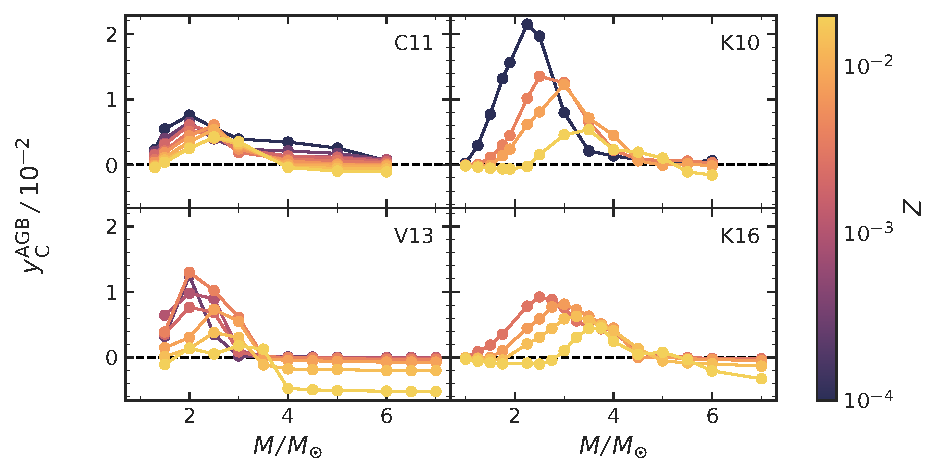
\includegraphics[scale=1]{agb_yields.pdf}
        \caption[]{The net fractional \agb\ C yield  plotted as a function of initial stellar mass $M$ and colour-coded according to metallicity. The black dashed line shows $\y=0$ for reference. Each panel represents yields from one of four \agb\ models: \cxi, \kx{}, \vxiii{}, \kxvi{} (see Section \ref{sec:agb} and  Appendix \ref{sec:oob_models}). }
        \label{fig:y_agb}
\end{figure*}

\begin{figure*}
    \centering
    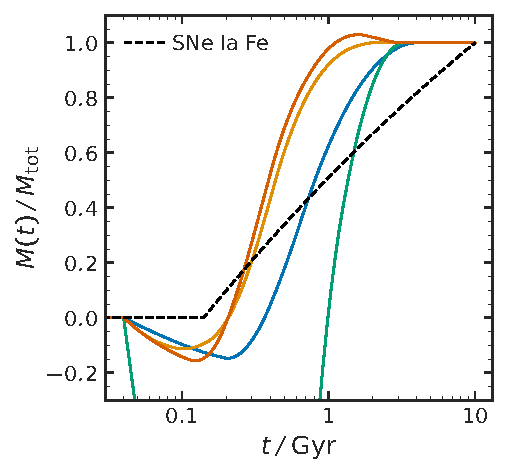
\includegraphics{y_agb_vs_t.pdf}
    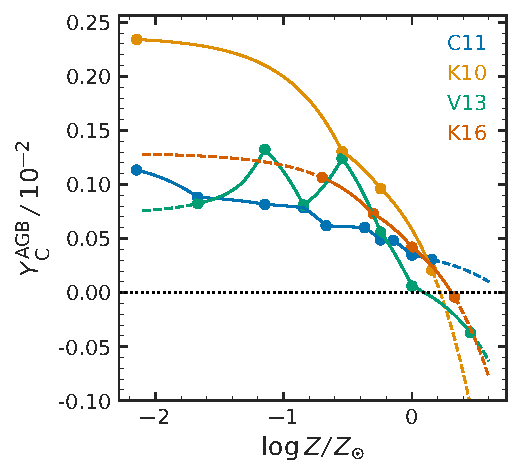
\includegraphics{y_agb_vs_z.pdf}

    \caption[]{ C production by \agb\ stars as a function of \ssp{} age, normalized to the total mass $M_{\rm tot}$ produced at $t=10$\,Gyr. \textbf{Left:} The four \agb\ yield models from literature at solar metallicity (\cxi, \kx{}, \vxiii{}, or \kxvi{}). The dashed black line shows the delay time distribution of type Ia supernovae ($\propto t^{-1.1}$) for comparison. \textbf{Right:} The (\imf-weighted) \agb\ C yield $\Ycagb$ as a function of metallicity for each of the \agb\ yield models. ($\Ycagb$ is the net mass of C produced by \agb\ stars per unit mass of star formation, after 10\,Gyr and assuming a \citealt{kroupa01} \imf.) }

    \label{fig:agb-ssp}

\end{figure*}



\subsection{Core Collapse Supernovae}


Massive stars form $^{12}$C in their cores through the triple--$\alpha$ process. However, only C ejected through supernovae and stellar winds contributes to the yield. 
While there are many stellar models providing predictions of \cc{} yields, the results of these models are highly uncertain due to the complexity of stellar modeling.

Fig.~\ref{fig:y_cc} plots calculations of the \imf-integrated yields, defined with Eq.~\ref{eq:imf-yield} (computed using \VICE's \texttt{vice.yields.ccsne.fractional} function). 
\cc{} models predict a wide range of C yields, spanning almost a factor of ten. 
Both the \citet{NKT13} and \cite{LC18} models show positive metallicity dependence. 
As metallicity increases, stars lose more of their mass to winds. In particular, C enriched envelop material is lost through winds before synthesized into heavier elements, so C yields can be strongly metallicity dependent (VERIFY).
Fig.~\ref{fig:y_cc} shows the \cxi{} \agb\ model for comparison on the left. Especially at $Z\approx Z_\odot$, most \cc{} models dominate \agb\ C production. Later, we will also show empirically this is the case.
The right of Fig.~\ref{fig:y_cc} shows the \cc{} [C/Mg] ratio for the different models, defined by
\begin{equation}\label{eq:c_mg_cc}
    {\rm [C/Mg]^{CC}} = \log_{10}\left( \frac{\Ycc}{\Yoc}\right) - \log_{10} \left( \frac{Z_{{\rm C},\ \sun }}{Z_{{\rm Mg},\ \sun }} \right).
\end{equation}
If only \cc{} produced C, then ${\rm [C/Mg]^{CC}}$ describes the equilibrium abundance of [C/Mg].
Different \cc\ models also span a large range in [C/Mg]. 
We chose to instead parameterize $\Ycc$ to simplify model inputs, as most \cc\ models fail to achieve near-solar [C/Mg].

Both rotation and explodability introduce substantial variations. The \cite{LC18} models include rotation, showing that variations in the rotational velocity of the star can dramatically increase the magnitude and metallicity dependence of $\Ycc$. Rotation induces more mixing allowing the CO core to grow larger and contributes to wind losses. As we will later show, \cc\ C production needs to be strongly metallicity-dependent at $Z/Z_\odot \approx 1$, which is consistent with the \cite{LC18} rapidly rotating models.
Assumptions about the explodability landscape affect C and Mg production. Increasing the fraction of stars that explode increases $\Ycc$, as stars that directly collapse do not contribute to explosive yields \citep{emily+21}. However, C is relatively unaffected by the black-hole landscape, as very massive stars contribute C through enriched winds. Since Mg is formed deeper in the core of \hms, the Mg yield drops much more steeply, so models where few stars explode (S16/W18) have higher [C/Mg].


O and Mg are both $\alpha$-elements, light elements produced in \cc{} through He-nuclei fusion. 
As we focus on constraining relative yields, we neglect O and Mg yield variations in the main text (excluding the uniform scaling of yields and massloading in Section~\ref{sec:outflows}). There is substantial variation in predicted Mg yields. 
Most models predict relatively flat trends metallicity (even with rotation as in \citealt{LC18}). 
However, the variation is significant and our adopted $\Yoc$ yield is much higher than most models, but O and Mg yields of \cc\ models do not fully match observations. \cc\ models underpredict $[{\rm Mg}/{\rm O}]$, and the reason why is unknown (see e.g. \citealt{emily+21}). Here, we assume ${\rm [O/Mg]} = 0$, which is not compatible with \cc\ models but is consistent with \apogee{} observations \citep{weinberg+19, weinberg+22}.
Because O and Mg are not perfectly identical in \apogee{}, the specific choice of $\alpha$-element may be a possible systematic.
    

\begin{figure*}
    \centering
    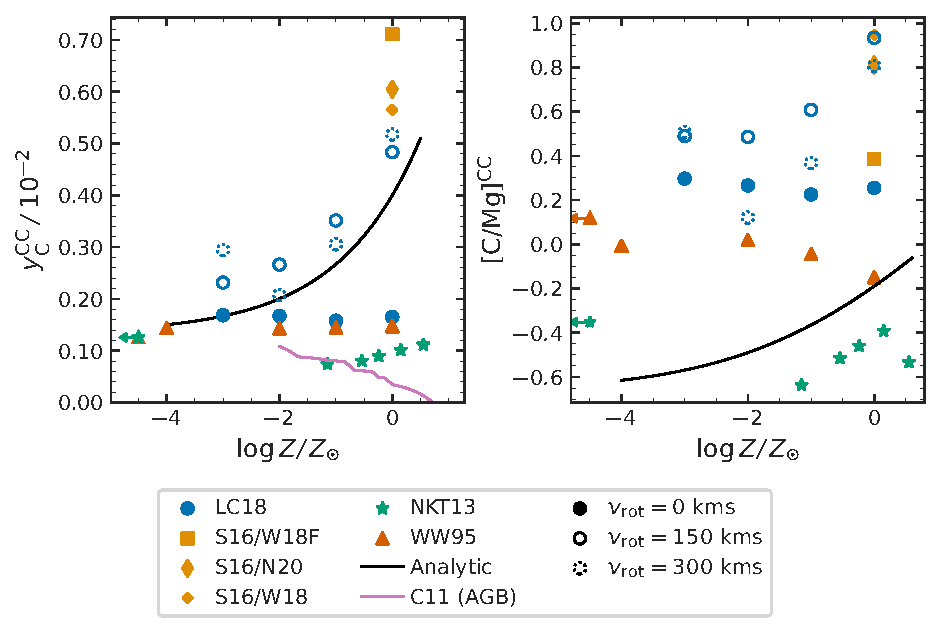
\includegraphics{cc_yields.pdf}
    \caption[High-Mass Star Carbon Yields]{
        C yields from high-mass stars.
        \textbf{Left} The \imf-weighted \cc\ yield of C as a function of metallicity.
        \textbf{Right} The \cc\ [C/Mg] abundance ratio, defined in Eq.~\ref{eq:c_mg_cc}. The black line is the derived C yield from Section \ref{sec:equilibrium},
    $\Ycc = 0.0028 + 0.001 (Z/Z_{\odot})$. Yields are shown for tables from 
    \citet[red triangles]{WW95}, \citet[orange squares and diamonds]{sukhbold+16}, 
    \citet[green stars]{NKT13}, and \citet[blue circles]{LC18}. \citet{sukhbold+16} report yields for different black hole landscapes, while \citet{LC18} provide yields at different rotational velocities.
    In the top panel, the pink line denotes $\Ycagb$ from \cxi{} for comparison. All models include wind yields. 
    (OUT OF DATE)
}
    \label{fig:y_cc}
\end{figure*}

\section{Analytic Approximations}
In this section, we describe approximations of galactic abundance trends and C yield models. While these are insufficient to describe the galaxy in full detail, we can use these simplified models to inform our investigation.

\subsection{Equilibrium Abundances}\label{sec:equilibrium}

Galaxies, when moderated by metal-poor gas accretion and feedback-driven outflows, reach a chemical equilibrium. The production of new metals is balanced by losses to new stars and outflows \citep{larson72, dalcanton07, FD08, PS11, lilly13}.
While our galaxy is likely not in perfect equilibrium or described by a single, homogeneous chemical
envirnoment, the equilibrium approximation is nevertheless useful in understanding yields and
metallicity dependence of solar neighborhood stars \citep[e.g.][]{james_dwarf,james+23,WAF17}. 

Here, we assume a simple \textit{one-zone} chemical evolution model \cite[e.g.][]{tinsley80, pagel09, matteucci21}.  Newly produced metals are homogeneously and instantaneously mixed, so this model evolves as a single, spatially-uniform chemical zone.
We define $M_{X}$ to be the mass of element $X$ in the gas-phase, $\dot{M}_\star$ to be the star formation rate (in $\Mo\,{\rm yr}^{-1}$), and $\eta$ to be the mass loading factor $\eta\equiv\dot{M}_{\rm outflow}/\dot{M}_\star$ (representing the strength of outflows). A \ssp\ returns a fraction $r$ of their birth mass to the interstellar medium, due to ejected stellar envelopes.%
\footnote{$r\approx0.4$ for a \citealt{kroupa01} \imf.}
Here, we will use $\alpha$ as a representative $\alpha$-element, such as O or Mg. 
Given the \imf-averaged yield $y_\alpha$, the rate of change in the gas-phase mass of $\alpha$ is a simple sum of sources and sinks,
\begin{equation} \label{eq:mdot_1}
    \dot{M}_\alpha =  y_\alpha\,\dot{M}_\star - \dot{M}_{\alpha,\,\text{remnants}} - \dot{M}_{\alpha,\,\text{outflows}}
\end{equation}
where $y_\alpha\,\dot{M}_{\star}$ describes \cc\ enrichment. 
In terms of the return mass fraction of stars $r$, the mass lost to remnants is $Z_\alpha\,\dot{M}_\star\,(1-r)$.  And, the outflows deplete mass at a rate $Z_\alpha \,\dot{M}_\star\,\eta$. (We assume the composition of outflows is the same as the interstellar medium.) With these definitions, Eq.~\ref{eq:mdot_1} is
\begin{equation}
    \dot{M}_\alpha= y_\alpha\,\dot{M}_\star - (1 + \eta - r)\,Z_\alpha\,\dot{M}_\star.
\end{equation}
Assuming an exponentially declining star formation history (\sfh{}) $\dot{M}_\star \propto e^{-t/\tau_{\rm sfh}}$, the equilibrium abundance is derived analytically by setting $\dot{Z}_\alpha=0$.
\begin{equation}\label{eq:z_eq}
    Z_\alpha^{\rm eq}(R) = \frac{y_\alpha}{1 + \eta(R) - r - \tau_\star / \tau_{\rm sfh}},
\end{equation}
where $\tau_{\star}$ is the star formation rate. ($\eta$ depends on $R$ to create a metallicity gradient. See also Section \ref{sec:vice} and Eq.~\ref{eq:eta_r}.)
In the special case of constant star formation, $\tau_{\rm sfh}\to\infty$, the denominator simplifies to $1+\eta-r$.

Likewise, for C production, where both \agb\ stars and \cc\ play a role,%
\footnote{In detail, the \agb\ contribution requires integration over the \sfh\ to account for the finite lifetimes of stars. However, for this exponential \sfh, this effect is minimal, so we simply use $\Ycagb$ for the current \agb\ contribution.}
Eq.~\ref{eq:z_eq} then becomes
\begin{equation}
    Z_{\rm C}^{\rm eq}(R) = \frac{\Ycc + \Ycagb}{1 + \eta(R) - r - \tau_\star / \tau_{\rm sfh}}
\end{equation}
The equilibrium C/$\alpha$ abundance ratio is then
\begin{equation}\label{eq:z_co}
    \frac{Z_{\rm C}^{\rm eq}}{Z_\alpha^{\rm eq}} = \frac{\Ycc + \Ycagb }{y_\alpha}.
\end{equation}
Analogous to \cite{james+23} arguments about N, the trends in abundance ratios are set by yield ratios in these \gce{} models. The effect of other \gce{} parameters (most importantly $\eta$) cancels. As a consequence, yield ratios should establish abundance ratio trends in models which assume a different normalization of element yields and mass-loading (see discussion below).
This argument can also be inverted to infer  yields from abundance ratio trends. To the extent that observed C and $\alpha$ trends reflect the equilibrium abundances in different Galactic regions, we can infer the total C yield.
\begin{equation}\label{eq:y_c_eq}
    \Ycc + \Ycagb =  y_\alpha \left(\frac{Z_{\rm C}}{Z_{\alpha}}\right)_\odot 10^{[{\rm C}/\alpha]}.
\end{equation}
As we know [C/$\alpha$] as a function of metallicity, Eq.~\ref{eq:y_c_eq} enables us to estimate both the magnitude and metallicity-dependence of $\Yct/y_\alpha$.
In Fig.~\ref{fig:analytic}, we show the inferred total C yields, based on this equation, and our best fitting linear model. From a linear regression, we suggest that
\begin{subequations}\label{eq:yc_inferred}
    \begin{align}
        \frac{\Yct(Z)}{y_{\rm O}} &\approx \frac{1}{3} + 4 \left(Z-\Zo\right) \\
        \frac{\Yct(Z)}{y_{\rm Mg}} &\approx 2.7 + 32 \left(Z-\Zo\right).
    \end{align}
\end{subequations}
These yield ratios results in an equilibrium abundance $[{\rm C}/\alpha] = -0.09$, which is consistent with the subgiant sample and is within \about{20\%} of the solar C/Mg mixture from \citet{asplund+09}.

\begin{figure}
    \centering
    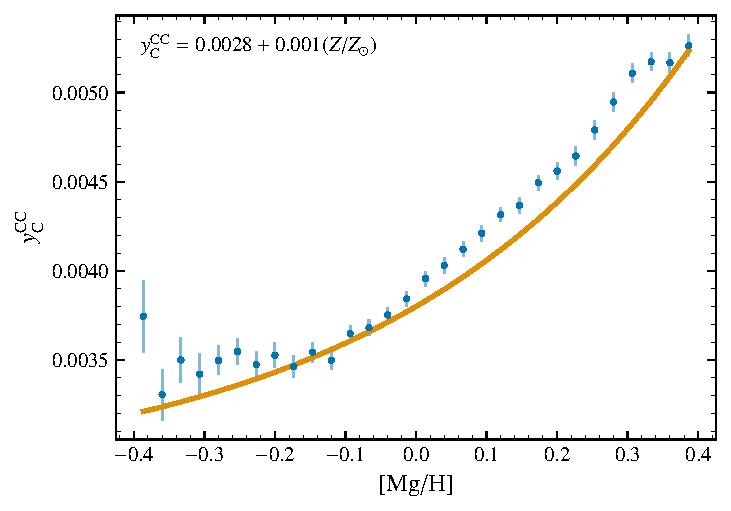
\includegraphics{analytic.pdf}
    \caption[]{Inferred high-mass star C yields as a function of metallicity. We assume equilibrium and $3\times {\rm C11}$ \agb\ yields (orange curve, see discussion in Section \ref{sec:equilibrium}). Blue points are the median value of $\Ycc$ for each bin in [Mg/H] with uncertainties based on the 16-84 percentile range.
    }
    \label{fig:analytic}
\end{figure}



\subsection{Analytic AGB}

To parameterize the \agb\ contribution to C production, we define $f_{\rm agb}$ to be the fraction of C which comes from \agb\ stars. 
\begin{equation}\label{eq:f_agb}
    f_{\rm agb} \equiv \frac{\Ycagb(Z=\Zo)}{\Yct(Z=\Zo)},
\end{equation}
In Section \ref{sec:agb_results}, we will show that $f_{\rm agb} \approx 0.2$. 
None of the \agb\ yield sets (\cxi{}, \kx{}, \vxiii{}, \kxvi{}) produce enough C relative to our total $\Ycc$ values. So, we introduce a normalization factor $\alpha_{\rm agb}$, which denotes a multiplicative scaling of $\Ycagb$ 
\begin{equation} \label{eq:alpha}
        \Ycagb \rightarrow \alpha_{\rm agb}\ \Ycagb.
\end{equation}
Table~\ref{tab:alpha_agb} contains the required values of $\alpha_{\rm agb}$ to reach $f_{\rm agb}=0.2$, the yields at solar metallicity, and the metallicity for each \agb\ yield set.

We can use the \caafe{} diagram of \apogee\ stars to estimate the delayed portion of C. When binned in metallicity, median [C/Mg] changes by about 0.25 dex across the range of [Mg/Fe]. As high-$\alpha$ stars have little to no delayed \ia\ Fe, these stars would also have little to no delayed \agb\ C. This means that AGB C stars make up about at most a fraction $f_{\rm agb} \approx 1 - 10^{-0.25} \approx 0.6$ of C production.

We also briefly explore an analytic \agb\ model, defined as a cubic piecewise in mass and linear in metallicity.
The piecewise is defined to have a maximum at $m_1$ and minimums at
the end points $m-\delta m_-$ and $m+\delta m_+$. The function becomes constant
outside of this range with (optionally) negative yields.
And the resulting equation (excepting a prefactor)

\begin{equation}
\y(m) = 
\begin{cases}
\y_0 & m \leq m_0 - \delta m_- \\
\y_1 + (\y_0 - \y_1)\; f\!\left(\frac{m_0 - m}{\delta m_-}\right) 
    & m_0 - \delta m_- < m \leq m_0 \\
    \y_1 + (\y_2 - \y_1)\; f\!\left(\frac{m - m_0}{\delta m_+}\right)
    & m_0 < m \leq m_0 + \delta m_+ \\
\y_2 & m_0 + \delta m_+ \leq m
\end{cases}
\end{equation}

where 
\begin{equation}
    f(x) = 3x^2 - 2x^3
\end{equation}

For the full equation, we take the above functional form multiplied by a
metallicity dependent term, so 

\begin{equation}
    \y_{\rm C}^{\rm agb}(m, Z) = \frac{\y(m)}{\int_1^8 m\,\y(m)\,{\rm IMF}(m)\;dm} 
    \left(\y_1 + \zeta \left(Z-\Zo\right) \right)
\end{equation}



\subsection{CCSNe Carbon Yields}
With the total C yield of Eq.~\ref{eq:yc_inferred} and given an \agb\ C yield, we can derive an observationally-consistant \cc\ C yield.
\begin{subequations}
    \begin{gather}
        \Ycc(\Zo) = \Yct(\Zo) - \Ycagb(\Zo)\\
        \zeta^{\rm cc} \equiv \frac{d\Ycc(\Zo)}{dZ} = \frac{d\Yct(\Zo)}{dZ} - \frac{d\Ycagb(\Zo)}{dZ}
    \end{gather}
\end{subequations}
This method reduces the number of free parameters of the model and enables all models to match \caah\ trends in \apogee{} subgiants when considering \agb\ yields with different metallicity dependences and normalizations. 
Table~\ref{tab:alpha_agb} contains our adaptive (regression-derived) values of $\zeta^{\rm agb}$ and $\Ycagb(\Zo)$. Table~\ref{tab:alpha_agb} also shows $\alpha^{\rm agb}_{20}$, the value of $\alpha^{\rm agb}$ required with our adopted total yields (Eq.~\ref{eq:yc_inferred}) to reach 20\% \agb\ C.

Our full \cc\ C yield model adds a low-metallicity enhancement term, which is insignificant at solar metallicities (e.g. thin disk stars) but enables models in Section~\ref{sec:gas} to match low-metallicity environments.
All-together, 
\begin{equation}\label{eq:zeta}
    \Ycc = y_{\rm C, 0}^{\rm cc} + \zeta^{\rm cc}\,(Z-\Zo) + \frac{2\,y_{\rm III}}{1 + Z/Z_{\rm III}}.
\end{equation}


\begin{table}
	\centering
    \caption[]{For each \agb\ yield set, the \imf-averaged \agb\ C yield at solar metallicity $y_{\rm C, 0}^{\rm agb}$ and the multiplicative factor reaches an \agb\ contribution of 20\% $\alpha_{\rm agb, 20}$. <UPDATE>}
	\label{tab:alpha_agb}
	\begin{tabular}{cccr} % four columns, alignment for each
		\hline 
    \agb\ Model & $y_{\rm C}^{\rm agb}(\Zo)$ & $\zeta^{\rm agb}(\Zo)$ 
                & $\alpha_{20}^{\rm agb}$\\
        \hline
        \cxi & 4.2E-4 & -0.022 & 2.9\\
        \kx & 6.5E-4 & -0.063 & 1.7\\
        \vxiii & 4.9E-4 & -0.032 & 16.5\\
        \kxvi & 5.6E-4 & -0.034 & 2.4\\
		\hline
	\end{tabular}
\end{table}






\subsection{Uncertainties}

We only perform this analysis on the \cxi{} yields because \cxi{} has yields tables more finely sampled in metallicity than the other three \agb\ yield tables. As the metallicity range of the data is small ($-0.4\lesssim {\rm [Mg/H]} \lesssim 0.4$), other models are more challenging to interpret in this range. Furthermore, the \apogee{} observations may have systematics. Other measurements of C abundances \citep[e.g.][]{vincenzo+21} have slight disagreements in the overall shape of the trend (see Section \ref{sec:jack}).
So, this expression of $\Ycc/\Yoc$ depends on the chosen \agb\ yield table, the \agb\ fraction, and the dataset. 
Additionally, these yields will be systematically biased if the galaxy is out of equilibrium, for example, due to a recent starburst \citep{mor+19,isern19}. Further exploration could investigate the magnitude of these uncertainties, but we find that the qualitative conclusions are similar despite substantial variations in the assumptions here.

As we will discuss in Section \ref{sec:outflows}, the normalization of yields and $\eta$ is degenerate. This can be observed in Eq.~\ref{eq:z_co}, where changes in $\eta$ or the scaling of $y_{\rm C}/y_{\rm Mg}$ would not affect equilibrium trends. Furthermore, in Eq.~\ref{eq:z_eq}, an increase in both $y_{\rm Mg}$ and $\eta$ would leave $Z_{\rm Mg}^{\rm eq}$ unchanged. Our models here are unable to distinguish the overall scaling of yields and outflow mass loading. Choosing to keep $y_{\rm C}$ fixed reduces unnecessary free parameters. So, at solar metallicity, we set


\section{The Multi-zone Model}\label{sec:vice}

Classical, \textit{one-zone} models of chemical evolution assume instantaneous mixing of metals in the star-forming interstellar medium \citep[e.g.][]{matteucci21}. This simple framework is a poor approximation of the Milky Way.  The Galaxy evolves \textit{inside-out}---where star formation is higher towards the center and in the early universe \citep{bird+13}. Additionally, stars can migrate several kpc over their lifetimes, mixing different chemical environments across the galaxy \citep{bird+12,sellwood+binney02}. For the rest of this paper, we focus on multi-zone models, which discretize the Galaxy into concentric rings in which stars move between.  
Our models extends the \citet[hereafter \JJ]{james+21} Milky Way model, run with the publicly available Versatile Integrator for Chemical Evolution (\VICE). 
This model is described extensively in \JJ~and concisely summarized  in \citet{james+23}. Here, we provide a brief overview of the relevant model components.

Star formation is treaded as follows. The Galaxy is divided into 200 rings, each 100\,pc wide. Each ring has a separate stellar population and gas supply. We initially assume an inside-out \sfh{}, where the star formation surface density $\Sigma_\star$ is given by 
\begin{equation}\label{eq:inside_out}
    \dot{\Sigma}_\star \propto \left(1-e^{-t/\tau_{\rm rise}}\right) e^{-t/\tau_{\rm sfh}}.
\end{equation}
$\tau_\text{rise}=2$\,Gyr describes when the star formation rate reaches a maximum, and $\tau_{\rm sfh}$ describes the decay timescale of star formation as a function of radius $R$. \JJ~derives $\tau_{\rm sfh}(R)$ through analysis of four integral field spectroscopy surveys in \cite{sanches20}. At each $R$, the \sfh{} is normalized to match the stellar surface density gradient \citep{BHG16} and the total stellar mass reaches $5.17\times10^{10}\,\Mo$ \citep{LM15}. Star formation ends beyond a radius $R=15.5\,$kpc. 
The gas inflow is calculated to maintain the \sfh{} for each radius and time, using an extension of a Kennicutt-Schmidt law \citep{kennicutt98},
\begin{equation}
\dot{\Sigma}_{\star} \propto 
\begin{cases}
    {\Sigma}_{\rm gas} & 2\times 10^7 \leq \Sigma_{\rm gas} \\ 
    {(\Sigma}_{\rm gas})^{3.6} & 5\times 10^6 \leq \Sigma_{\rm gas} < 2\times10^7 \\ 
    {(\Sigma}_{\rm gas})^{1.7} & \Sigma_{\rm gas} < 5\times10^6 \\ 
\end{cases}
\end{equation} 
where $\Sigma_{\rm gas}$ is measured in \Mo\,kpc$^{-2}$. 
The scaling of this relationship varies with time due to the redshift dependence of $\tau_\star$ in molecular gas observed by \citet{tacconi18}. We assume a \citet{kroupa01} \imf.


To account for radial migration, \JJ\ used the \texttt{h277} hydrodynamical
simulation results \citep{christensen12, zolotov12, loebman12, BZ14}. Simulation parameters are described in \citet{bird+21}. 
Each \VICE\ single stellar population (SSP) is matched to an \textit{analog} in \texttt{H277}, chosen to form at a similar time and radius $R$. By taking the change in radius $\Delta R$ of the analogs, the SSPs move to their final radii with a $\sqrt{\text{time}}$ dependence.
The $\Delta R \propto \sqrt{\rm time}$ dependence arises when migration proceeds as a consequence of the diffusion of angular momentum \citep{frankel18, frankel20}.
We do not account for radial gas flows.
Using the results of a hydrodynamical simulation without modification limits the free parameters in the model; however, we am limited to one dynamical history. 
We do explore a normal-distribution random walk migration based on \citet{frankel18}, without noticeable impacts on our results. All models shown here use the \texttt{h277}-based migration. The full impact of the details of a galaxy's dynamical history on its chemical evolution is still unknown.

As the strength of outflows controls the resulting $\alpha$-element abundances, \JJ~create a metallicity gradient by defining
\begin{equation}\label{eq:eta_r}
\eta(R) = r - 1 + \frac{y_{\alpha}^{\rm CC}}{Z_{\alpha, \odot}} 10^{(-0.08\,\text{kpc}^{-1})(R-4\,\text{kpc})+0.3}.
\end{equation}
This choice of $\eta(R)$ results in a [$\alpha$/H] gradient consistent with Milky Way observations \citep[e.g.][]{hayden+14, weinberg+19, frinchaboy+13}.


\section{Results}
\subsection{Data Selection}


Subgiants provide the ideal observational constraint to our model. 
When a star enters the Red Giant Branch (RGB), material from the CNO-processed core is mixed with the envelope in first dredge up, enhancing N and depleting C \citep{iben67, vincenzo+21,KL14}. RGB stars thus require model-dependent corrections to recover surface abundances \citep[e.g.][]{vincenzo+21}. On the other hand, gravitational settling can affect main sequence stellar abundances \citep[e.g.][]{souto19}. Subgiants have well-mixed envelopes, so gravitational settling is not as significant, and subgiants have not yet experienced first dredge up. We use a sample of \apogee\ DR17 stars \citep{apogee17} as selected in \citetjack. We only compare the models to the low-$\alpha$ sequence (representing the thin disk) unless otherwise specified.  The selection criteria and differences between the samples are described in more detail in Appendix~\ref{sec:jack}.



\subsection{Evolution of Carbon Abundances}

Here, we present the time evolution of our fiducial model. In the next sections, we will discuss the choice of parameters and agreement with observations. 
The fiducial model has the following qualitative characteristics of its C yields.
\begin{description}
    \item C is mostly (\about{80\%}) produced in \cc
    \item \cc\ produce more C at higher metallicities
    \item \agb\ stars produce less C at higher metallicities 
\end{description} 
The fiducial model uses the \cxi{} \agb\ yield tables uniformly scaled by a factor of 2.9 (see Section \ref{sec:agb}, and Table \ref{tab:fiducial_mod}). 

Fig.~\ref{fig:c_evo} shows time evolution tracks of the fiducial model for \caah\ and \caafe. 
As discussed in Section~\ref{sec:equilibrium}, \caah\ is set by the total C/Mg yields. 
\caafe\ is instead useful in understanding delayed C production. 
As both Fe and C are delayed elements, [Mg/Fe] steadily decreases after a star formation event, unlike [Mg/H] which quickly reaches equilibrium.  All plots showing \caafe\ going forward are selected in metallicity such that $-0.15 \leq {\rm [Mg/H]} \leq -0.05$, so metallicity-dependent yields do not affect this plot. 
The \caafe{}-diagram is, in essance, an emperical delay-time-distribution for a single stellar population of C, especially as we assume a $\propto t^{-1.1}$ delay-time-distribution for Fe. 
Comparing the top and bottom panels of Fig.~\ref{fig:c_evo} highlights the differences between \caah\ and \caafe. While \caah\ quickly reaches its final equilibrium distribution (within \about{5}\,Gyr), \caafe\ continues to evolve in both [Mg/Fe] and [C/Mg] until the simulation ends.

C evolution proceeds as follows, (for a single zone)
\begin{enumerate}
    \item \cc\ initially dominate production. As $\Ycc$ has strong metallicity dependence, [C/Mg] increases with time. 
    \item \agb\ stars contribute delayed C, causing [C/Mg] to increase even faster with [Mg/H]. 
    \item{} [C/Mg] plateaus as C also approaches equilibrium. 
    \item{} [C/Mg] may decrease due to declining SFH or slightly negative yields from \about{1}\,\Mo stars.

\end{enumerate}


\begin{figure*}
\centering
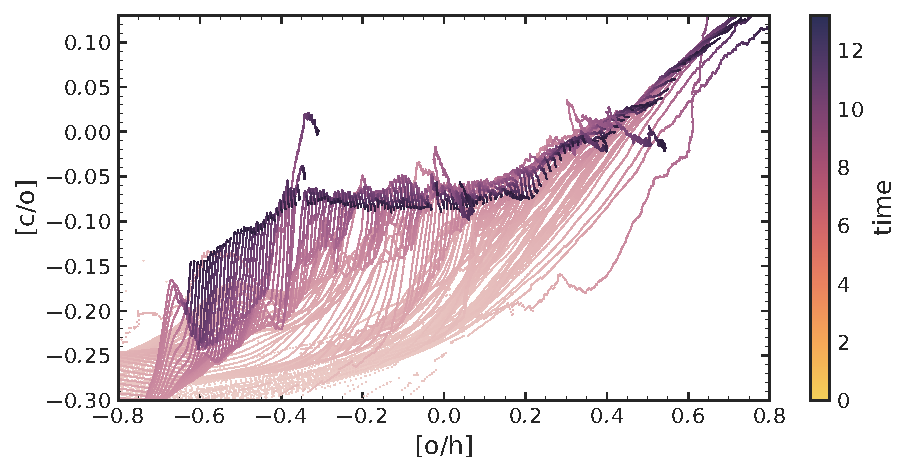
\includegraphics{all_the_tracks.pdf}
\caption[]{
    Time evolution of gas-phase C abundances in our fiducial model.
    Each line represents a zone at a different galactic radii. The lines are coloured-coded by time. The left shows \caah\ and the right \caafe. We artificially restrict the axis range in each case to better see solar-annulus and present-day evolution.
    <UPDATE, CHECK LEFT?RIGHT USAGE>
}
\label{fig:c_evo}
\end{figure*}

Fig.~\ref{fig:f_agb_evo} shows $f_{\rm agb}$ calculated from the fiducial model of current effective C yields in the gas phase (using the SFH as a proxy for $\Ycc$. 
At early times, \cc\ dominate. As the galaxy evolves, \agb\ have time to add C, increasing $f_{\rm agb}$. However, the metal-rich inner regions lower \agb\ C yields, so these regions never reach as high of a $f_{\rm agb}$ as the outer regions do. 

\begin{figure}
    \centering
    \includegraphics{f_agb_rt.pdf}
    \caption[]{The evolution of $f_{\rm agb}$ across the Galaxy and with time.}
    \label{fig:f_agb_evo}
\end{figure}




\subsection{High-Mass Stellar Yields}\label{sec:results_highmass}

\cc, which likely make up the majority of C, set the overall C abundance trends.
 Fig.~\ref{fig:first_models} shows models with varying $\Ycc$ metallicity dependence. As the \caah~trend is approximated by equilibrium trends, the models with stronger metallicity dependence have a stronger slope in \caah. 
 However, \caafe~is minimally affected by these changes since \cc\ occurs on much shorter timescales than \ia\ and \agb\ enrichment. The only effects on \caafe, when considering the narrow metallicity slice, are because of either the slight change in equilibrium abundances, the imperfect evolution of the galaxy, or that the interstellar medium abundances are set by stars which were born at poorer metallicities. 
 Hence, \caah\ tells us about the total C yield with metallicity, which \caafe\ is independent of. If we know the \agb\ C yields, then with observed \caafe\ abundance trends, we can infer the \cc\ C yields with metallicity.


\begin{figure*}
\includegraphics{all_p1.pdf}

\caption[]{
    Stellar abundance trends in our model, assuming metallicity independent $\Ycc$. Colored lines quantify the median [C/Mg] in bins of [Mg/H] for our four \agb\ yield models from the literature (see Section \ref{sec:agb}). Black points and grey dashes represent the median and standard deviations of [C/Mg] for each [Mg/H] bin in the \citetjack~sample. In the right panel, we show the trends only for stars where $-0.15\leq {\rm [Mg/H]}\leq -0.05$.
}
\label{fig:first_models}
\end{figure*}

\subsection{Low-Mass Stellar Yields}\label{sec:agb_results}

\caafe\ is sensitive to the assumptions about delayed C from \agb\ stars. If no C comes from low-mass stars, then [C/Mg] would be independent of [Mg/Fe], only [Mg/H]. Instead, C shows strong trends  in \caafe\, independent of metallicity. 

In Fig. <REF>, we first show the four C yield models (\kx, \kxvi, \cxi, \vxiii). For the most part, the \agb\ yield sets result in qualitatively similar predictions. \vxiii, however, does not reproduce solar trends as the model predicts strong C production at slightly above solar metallicities, resulting in a decreasing [C/Mg] with [Fe/Mg]. 
As all \agb\ models predict some low-mass C destruction, each model does predict a downturn in [C/Mg] as [Fe/Mg] increases. A recent burst in star formation may hide this downturn (see NEXT SECTION), but the C destruction is not supported directly by observations. 




Here, we investigate adjustments to the \agb\ yield fraction $f_{\rm agb}$
Fig.~\ref{fig:f_agb} shows three models with different \agb\ fractions while using \cxi{} yields.  The \caafe~relationship is set by $f_{\rm agb}$ because a specific amount of C must be released at a delayed time to match the \ia\ production of Fe and increase [C/Mg] as [Mg/Fe] decreases to reproduce the data.
Increased $f_{\rm agb}$ results in a decreased slope in \caah, owing to the negative metallicity dependence of $\Ycagb$. So while \caah~alone cannot differentiate models which vary $f_{\rm agb}$ and $\zeta$ correspondingly, \caafe~provides information on $f_{\rm agb}$. So, we can use \caafe~to estimate $f_{\rm agb}\approx 0.2$, and then choose $\zeta$ to match \caah.



Negative \agb\ yields cause a morphological change in the abundance trends. If the yields of low mass stars are negative, then at late times in a SSP, C abundances will decrease. This will appear as a downturn in the \caafe{} abundance trends as [Mg/Fe] approaches solar values. As we do not observe this in the data, this is either obscured by \sfh\ (Seee eeee) or observational scatter. 
Instead, if lower-intermediate mass \agb\ stars produce negative carbon yields, it is possible to observe this as a dip in the early parts of the \caafe{} trend...



\begin{figure*}
\centering
\includegraphics{all_p2.pdf}

\caption[]{Similar to Fig.~\ref{fig:first_models}, except where the \agb\ C contribution is varied from the fiducial ($f_{\rm agb}=0.2$) to 0.1 and 0.3 (see Eq.~\ref{eq:f_agb} and Section.~\ref{sec:agb_results}.}
\label{fig:caafe_agbs}
\end{figure*}





\subsection{Star Formation History} \label{sec:sfh}

In this section, we consider two modifications of our fiducial \sfh{}: \textit{lateburst} and \textit{earlyburst}.
Our lateburst model adds a Gaussian factor to the inside-out \sfh{},
\begin{equation}\label{eq:lateburst}
    \dot{\Sigma}_\text{lateburst} \propto \dot{\Sigma}_\text{inside-out} \left(1 + A\,e^{-(t-\tau_{\rm burst})^2/2\sigma^2_{\rm burst}} \right)
\end{equation}
where $A=1.5$ represents the amplitude of the birth, $\tau_\text{burst}=10.8$\,Gyr is the time where the burst is strongest, and $\sigma_\text{burst}=1$\,Gyr is the width of the burst.
Our earlyburst model instead >>>>>?????  at $t_1=5$\,Gyr. 
\begin{equation}\label{eq:twoinfall}
    \dot{\Sigma}_{\rm earlyburst} \propto A\,e^{-(t-t_1)/\tau_{\rm burst}} + 
\begin{cases}
    \left(1-e^{-t/\tau_\text{rise}}\right)e^{-t/\tau_\text{rise}} & t_1 < t \\
      0 & t<t_1
\end{cases}
\end{equation}
where we take the burst duration, $\tau_{\rm burst}=1$\,Gyr.
This approximately corresponds to the Gaia-Encelidus merger, inducing higher star formation in the Milky Way \citep{spitoni21, bonaca20, helmi18}.

Fig.~\ref{fig:sfh_models} shows three models with these alternate \sfh{}. Changes to the \sfh{} leave \caah\ unchanged, but they do introduce slight variation in \caafe. Models with higher \agb{} fractions are more sensitive to variations in the \sfh{}. The late burst models result in [C/Mg] continuing to increase at low [Mg/Fe], but also introduce a dip not present in the data. Additionally, the early-burst
reproduces the slight break between the low and high $\alpha$ sequences, but overshoots equilibrium more severely than the fiducial model. 
In general, any of these \sfh{}s are consistent with this model.



\subsection{Degeneracies} \label{sec:outflows}


\gce{} models of the Milky Way fall into two classes---those which incorporate significant mass-loading (e.g., this work) and those which neglect mass-loading but lower effective yield to match observed abundances \citep[e.g.][]{MCM13, MCM14, spitoni19, spitoni20, spitoni21}.
An increase in stellar yields has a nearly identical effect as a decrease in the mass-loading factor $\eta$ (see Appendix B of \citealt{james_dwarf}).
The equilibrium arguments discussed in Section \ref{sec:equilibrium} suggest however that abundance ratios are independent of the choice of normalization and the value of $\eta$. We, therefore, expect our results regarding the relative yield $y_{\rm C}/y_{\rm Mg}$ and its metallicity dependence to extend to the other class of models omitting mass loading. We demonstrate this further here.

The theoretical motivation for decreasing yields is the uncertainty in stellar explodability.
If fewer \hms\ explode, then the yields will be reduced by some factor. Additionally, some fraction of supernovae ejecta may be lost directly to an outflow, lowering effective yields. To explore reduced outflow models, we lower both $\eta$ and all yields by the same factor to leave the equilibrium abundances unchanged. 

Fig.~\ref{fig:eta} shows models with variations of the mass loading strength. While changing the value of $\eta$ affects the metallicity distribution of stars, all of the models in Fig.~\ref{fig:eta} still evolve along the same path. Our model is unable to differentiate a uniform decrease in both outflows and yields.

An addition source of theoretical uncertainty in this result is that the \ia\ yield and delay time distributions have their own uncertainties. We discuss variations in $y_{\rm Fe}^{\rm Ia}$ in NOWHERE, and find that the qualitative conclusions are largely unaffected. We, therefore, focus on the choices of $y_{\rm Fe}^{\rm Ia} = 0.00214$ and a $t^{-1.1}$ delay time distribution choices from the fiducial model here.
In short, the scaling of the trend and metallicity dependence of C (as seen in
the \caah\ trend) gives information on the total C yield and the behavior of \cc\ (as the dominating producer of C), the \caafe\ trend exposes the delayed effect of C from \agb\ contribution.




\subsection{Gas-Phase Abundances}\label{sec:gas}

As a final test of the model, we compare the model predictions against gas-phase measurements. Fig.~\ref{fig:gas_phase} shows the fiducial model's gas-phase predictions compared to observations of the Milky Way and extragalactic HII regions, halo stars, and damped Lyman-alpha systems. 
While obervations in HII regions and Milky Way stars agree that C/O generally increases at near-solar metallicities, damped Lyman-alpha systems and metal poor stars imply that C/O may also increase again at very low metallicities. 



Measurements of C abundances are challenging. 
In HII regions, C/O abundance ratios are measured with either recombination lines or collisional excitation lines. However C lacks strong collisional excitation lines, and recombination lines fall in the ultraviolet without nearby reference H lines \citep{skillman+20}. Additionally, recombination and collisional excitation measurements disagree by a factor of \about{2} \citep{GR07}. 
While broad consistancy of our model with gas-phase measurments is nice, the large measurment errors limit the evaluative power of HII regions.
We additionally include Milky Way thick disk (high-$\alpha$) and halo stars, which span a larger range of metallicities than thin disk stars. However, metal-poor abundance measurments require consideration of 3D-NLTE effects (e.g. CITE). 
Finally, dwarf galaxies, damped Lyman-alpha systems, and extragalactic regions may represent different \sfh{}s than the Milky Way.
As \agb\ C production is sensitive to variations in the \sfh, these environments may not exactly match our subgiant sample, limiting the usefulness of these abundance measurments in evaluating our model.


Fig.~\ref{fig:gas_phase} shows the single-zone model and time-slices of the fiducial multi-zone model at present day and $t=2$\,Gyr. 
Here, we consider a single-zone model with parameters consistant with the Gaia-Encelidus sausage\footnotemark{}. We chose the model to have outflows $\eta=6$, star formation efficiency $\tau_{\star}=9\,{\rm Gyr}$, and a star formation history $\propto e^{-t/2{\rm\,Gyr}}$, evolved for 6\,Gyr. 
The single-zone model is better able to replicate the slope of the abundances in dwarf galaxies, HII-regions, and halo stars. The single-zone model is an evolutionary track, whereas the multi-zone models moreso show equilibrium tracks. As the single-zone model also evolves slower, the late contribution of AGB stars causes the steeper slope at near-solar metallicities. By including an increase of C yields at low-metallicity, the single-zone model is also able to reproduce the increasing [C/O] abundances with decreasing metallicity past ${\rm [O/H]} < -1.5$.
In any case, there is large scatter in the measurments, which both models fall within.



\footnotetext{See e.g. CITATION. Th Gaia-Encelidus sausage (GSE) is a kinematically and chemically distinct group of halo stars consistant with the merger of a dwarf galaxy early in the Milky Way's formation.}


\begin{figure*}
\centering
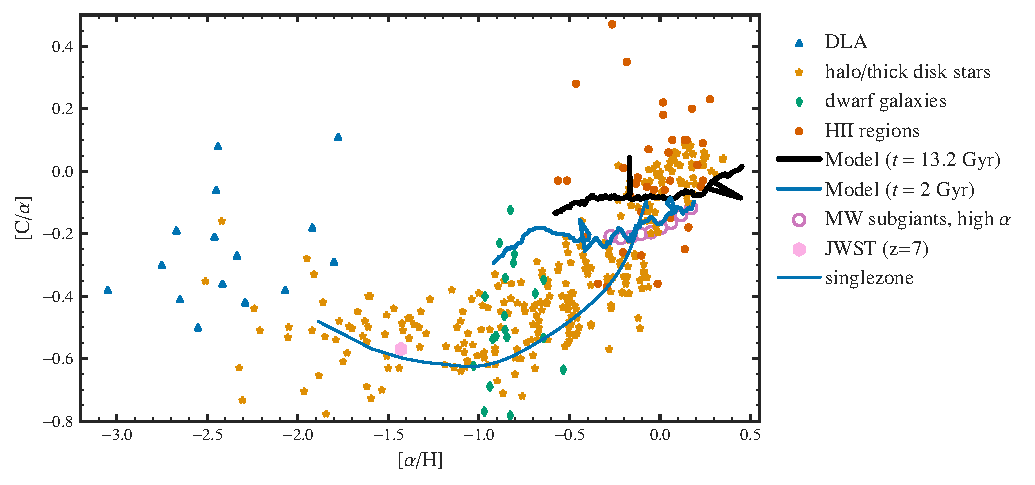
\includegraphics[]{summary.pdf}
\caption[]{Gas-phase C abundances. We plot our model at $t=2$\,Gyr and present day as thick solid lines. Points represent measurements in 
    HII regions    \citep[pink circles;][]{skillman+20, esteban+02, esteban+09, esteban+14, esteban+19}
    damped Lyman-alpha (DLA) systems \citep[blue triangles;][]{ellison+10, srianand+10, dutta+14, DZ+03, pettini+08, morrison+16,cooke+17},  % a1: Cooke et al. (2015); 2: Dutta et al. (2014); 3: Cooke et al. (2014); 4: Ellison et al. (2010); 5: Cooke et al. (2011b); 6: This work; 7: Pettini et al. (2008); 8: Morrison et al. (2016); 9: Srianand et al. (2010); 10: Cooke et al. (2012); 11: Dessauges-Zavadsky et al. (2003)
    dwarf galaxies \citep[red diamonds;][]{berg+19},
    Milky Way halo and thick disk stars \citep[green stars;][]{nissen+14, fabbian+09},
    and Milky Way high-$\alpha$ stars (yellow points; \citealtjack).
    (OUT OF DATE)
}
\label{fig:gas_phase}
\end{figure*}


\section{Conclusions}

In this work, we investigated the role of C yields on the predictions of multi-zone \gce{} models. 
We began by adopting an equilibrium approximation to estimate the total C yields with metallicity from \apogee{} subgiant \caah{} trends.
We find that <EQUATION>.
We show that \caah{} is a diagnostic for total C yields with metallicity, but \caafe{} provides information about delayed C production. From the \caafe{} trends, we estimate that \agb\ stars contribute \about{20\%} of total C abundances, with 1--3\,\Mo the most importaint. In this model, the remaining \about{80\%} of C comes from high-mass stars with a metallicity dependent yield of $\Ycc/\Yoc=<\text{EQUATION}>$, broadly consistant with rotating \cc\ models.

We additionally explore variations of the assumed \sfh{} and outflow mass-loading factor $\eta$. We find that alternate \sfh{}s can slightly affect \caafe, but \caah~is mostly unaffected. Decreasing both outflows and yields by the same factor leaves the \caah~and \caafe~trends unaffected, ingoring effect to the metalliticy distribution of starrs. These constraints on the relative yields of C, O, and Mg are robust against variations in $\eta$.

Finally, we compare our model against gas-phase measurements and Milky Way halo stars. By including yields which are enhanced at low metallicities, \cc\ and \agb\ stars together are able to explain the general trends of C from metallicities of -3 to 0.5. 

These C yield constraints provide a useful benchmark for stellar evolution models. C yields are sensitive to poorly understood processes, including mass-loss prescriptions, explodability, nuclear cross sections, convection, and stellar structure. Future spectroscopic surveys combined with Gaia kinematics \citep{gaia} will continue to enhance our understanding of chemical evolution. Both the Sloan Digital Sky Survey V's Milky Way Mapper program ({\sc SDSS-V/MWM}) \citep{sdssv} and the Dark Energy Spectroscopic Instrument ({\sc DESI}) Milky Way survey \citep{desi, desi:mw} will each measure spectra of upwards 6,000,000 Milky Way stars. These larger samples will enable similar work to tighten constraints on stellar models and our understanding of galaxy structure and evolution.



%%%%%%%%%%%%%%%%%%%%%%%%%%%%%%%%%%%%%%%%%%%%%Log in with your OSC username and password.

%%%%%
\section*{Acknowledgements}

 Here you can thank helpful
colleagues, acknowledge funding agencies, telescopes and facilities used etc.
Try to keep it short.

Software that has contributed to this work included  
\VICE~\citep{JW20, james+21},
\textsc{matplotlib} \citep{matplotlib},
\textsc{scipy} \citep{scipy},
\textsc{IPython} \citep{ipy},
\textsc{pandas} \citep{pandas},
\textsc{numpy} \citep{numpy},
\textsc{astropy} \citep{astropy:2013, astropy:2018, astropy:2022},
and 
\textsc{seaborn} \citep{seaborn}
.
Additionally, we thank \citet{OhioSupercomputerCenter1987} for the use of its facilities for the simulations. 


%%%%%%%%%%%%%%%%%%%%%%%%%%%%%%%%%%%%%%%%%%%%%%%%%%
\section*{Data Availability}

 
The inclusion of a Data Availability Statement is a requirement for articles published in MNRAS. Data Availability Statements provide a standardised format for readers to understand the availability of data underlying the research results described in the article. The statement may refer to original data generated in the course of the study or to third-party data analysed in the article. The statement should describe and provide means of access, where possible, by linking to the data or providing the required accession numbers for the relevant databases or DOIs.


%%%%%%%%%%%%%%%%%%%% REFERENCES %%%%%%%%%%%%%%%%%%
\bibliographystyle{mnras}
\bibliography{main}


%%%%%%%%%%%%%%%%% APPENDICES %%%%%%%%%%%%%%%%%%%%%

\appendix


\section{The Subgiant Sample}\label{sec:jack}

As the primary observational constraint, we use the criteria outlined in \citetjack~to create a sample of subgiant from \apogee{} DR17 \citep{apogee17}. apogee is part of the Sloan Digital Sky Survey and measures high-resolution spectra of thousands of stars \cite{sdss17}. Chemical abundances are determined from the \apogee\ Stellar Parameter and Chemical Abundance Pipeline ({\sc aspcap}) \citep{aspcap}.  


Photospheric C and N abundances in subgiant are reflective of their birth abundances \citep{gilroy89, korn+07, lind+08, souto+18, souto19} As first dredge up, which affects C and N abundances, only occurs during the ascent onto the RGB, subgiant stars are unaffected by this enrichment. 

An alternate approach for this analysis would be to estimate the birth abundances of RGB stars by correcting surface abundance effects from first dredge up as in \cite{vincenzo+21}. Subgiants are the more attractive option since these observations do not rely on model-dependent corrections. However, RGB stars are more luminous, potentially allowing better coverage of the Galactic disk.


We choose to use \citetjack\ sample as this does not rely on additional layers of modeling, providing a more direct constraint to our model and limiting our systematic uncertainties.



Fig.~\ref{fig:subgiant_selection} shows a plot of all \apogee\ stars and the \citetjack polygon selection criteria. 
 \citetjack~select a region of stars based on surface gravity $\log g$, and effective surface temperature, $T_\text{eff}$.
 \begin{equation}
    \begin{cases} \label{eq:subgiant_selection}
        \log \text{g} \geq 3.5 \\
        \log \text{g} \leq 0.004\,T_{\rm eff} - 15.7 \\
        \log \text{g} \leq 0.000706\,T_{\rm eff} + 0.36 \\
        \log \text{g} \leq -0.0015\,T_{\rm eff} + 12.05 \\
        \log \text{g} \geq 0.0012\,T_{\rm eff} - 2.8. \\
    \end{cases}
\end{equation}
Additionally, we included stars in \apogee{} marked by the following flags.
\begin{itemize}
\item \verb|APOGEE_MIRCLUSTER_STAR|
\item \verb|APOGEE_EMISSION_STAR|
\item \verb|APOGEE_EMBEDDEDCLUSTER_STAR|
\item \verb|young cluster (IN-SYNC)|
\item \verb|APOGEE2_W345|
\item \verb|EB planet|
\end{itemize}
This cut isolates a clean sample of \about{12,000} subgiants.
We furthermore isolate the low- and high-$\alpha$ sequences with the cut
\begin{equation}\label{eq:high_alpha}
\begin{cases}
\text{[Mg/Fe]} >0.12-0.13\,\text{[Fe/H]}, & \text{[Fe/H]}<0\\
\text{[Mg/Fe]} >0.12, & \text{[Fe/H]}>0. \\
\end{cases}
\end{equation}
The low-$\alpha$ sequence is better reproduced by this model, so we use this cut of the subgiants to compare the models against except for comparing \caafe. 




\begin{figure}
    \centering
    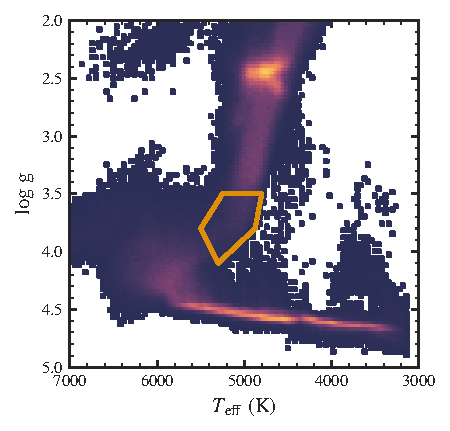
\includegraphics{logg_jack.pdf}
    \caption[]{
        A Kiel diagram of \apogee{} stars. Following \citetjack, we select subgiants in the orange polygon (see Equation \ref{eq:subgiant_selection}). These stars have not yet experienced first dredge-up, so their photospheric C and N abundances should reflect their birth mixture.
    }
    \label{fig:subgiant_selection}
\end{figure}



\section{\agb\ Yield Models} \label{sec:oob_models}
A brief summary of the four \agb\ models we consider, the masses and metallicites of each yield set, and differences between the models.

\hypertarget{C11}{\texttt{C11}}. 
Yields from \citet{cristallo+11,cristallo+15}. 
Models include masses 1.3, 1.5, 2.0, 2.5, 3.0, 4.0, 5.0, and 6.0 \Mo; and 
metallicities $Z = $ 0.0001, 0.0003, 0.001, 0.002, 0.003, 0.006, 0.008, 0.01, 0.014, 0.02. 

\hypertarget{K10}{\texttt{K10}}.
Yields are published in \citet{karakas10}. 
Models include masses  1.0, 1.25, 1.5, 1.75, 1.9, 2.25, 2.5, 3.0, 3.5, 4.0, 4.5, 5.0, 5.5, 6.0 \Mo;
and metallicities $Z=$ 0.0001, 0.004, 0.008, 0.02. 

\hypertarget{V13}{\texttt{V13}} 
Yields are published in \citet{ventura+13,ventura+14,ventura+18,vincenzo+21}, 
Models include masses 1.5, 2.0, 2.5, 3.0, 3.5, 4.0, 4.5, 5.0, 6.0, 6.5, 7.0 \Mo; 
and metallicities $Z=$ 0.0003, 0.001, 0.002, 0.004, 0.008, 0.014, 0.04.
\vxiii is evololved with DHFJKSLDF,
\vxiii is unusual in that hot bottom burning is much stronger than other models, resulting in much lower stellar yields and negative yields above solar metallicities.


\hypertarget{K16}{\texttt{K16}} 
Yields are published in \citet{KL16,karakas+18}
Models include masses 1.0, 1.25, 1.5, 1.75, 2.25, 2.5, 2.75, 3.0, 3.25, 3.5, 3.75, 4.0, 4.5, 5.0, 5.5, 6.0, 7.0 \Mo; 
and metallicities $Z=$ 0.0003, 0.001, 0.002, 0.004, 0.008, 0.014, 0.04.
This yield set was extended up to metallicities of 0.1 in DFJSD; however, we do not consider this range here.


\begin{figure}
    \centering
    \includegraphics{apogee_caafe_binned}
    \caption{hello}
    \label{fig:caafe_binned}
\end{figure}


\bsp	% typesetting comment
\label{lastpage}
\end{document}




